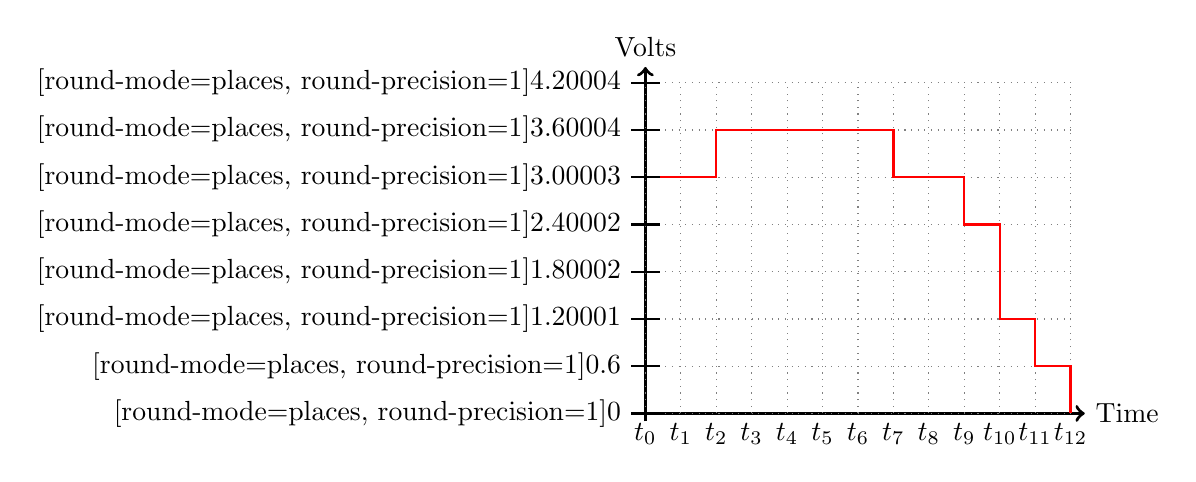
\begin{tikzpicture}[xscale=.9]
		% axes
    	\draw[->, very thick] (-0.1,0) -- (6.2,0) node[right] {Time};
    	\draw[->, very thick] (0,-.1) -- (0,4.4) node[above] {Volts};

		% samples
		\draw[xstep=.5, ystep=.6, thin, color=gray, dotted] (0,0) grid (6, 4.2);

		% discrete
		\draw[thick, color=red]
		(0, 3)
		-- (.5, 3) -- (1, 3)
		-- (1, 3.6) -- (1.5, 3.6) -- (2, 3.6) -- (2.5, 3.6) -- (3, 3.6) -- (3.5, 3.6)
		-- (3.5, 3) -- (4, 3) -- (4.5, 3)
		-- (4.5, 2.4) -- (5, 2.4)
		-- (5, 1.2) -- (5.5, 1.2)
		-- (5.5, 0.6) -- (6.0, 0.6)
		-- (6.0, 0);

		% xtics
		\foreach \x in {0, ..., 12}
		{
			\draw ({\x/2}, 0) node[below] {$t_{\x}$};
		}

		% ytics
		\foreach \y in {0, 0.6, ..., 4.3}
		{
			\draw[thick] (.2, \y) -- (-.2, \y) node[left] {\num[round-mode=places, round-precision=1]{\y}};
		}
\end{tikzpicture}
